\documentclass{article}
\usepackage[utf8]{inputenc}
\usepackage[T1]{fontenc}
\usepackage{graphicx}
\usepackage{amsmath}
\usepackage[textwidth=160mm, textheight=220mm]{geometry}

\begin{document}
\title{Single-track odometry with two wheel encoders}
\maketitle

\parbox{.55\textwidth}{%
\begin{center}
  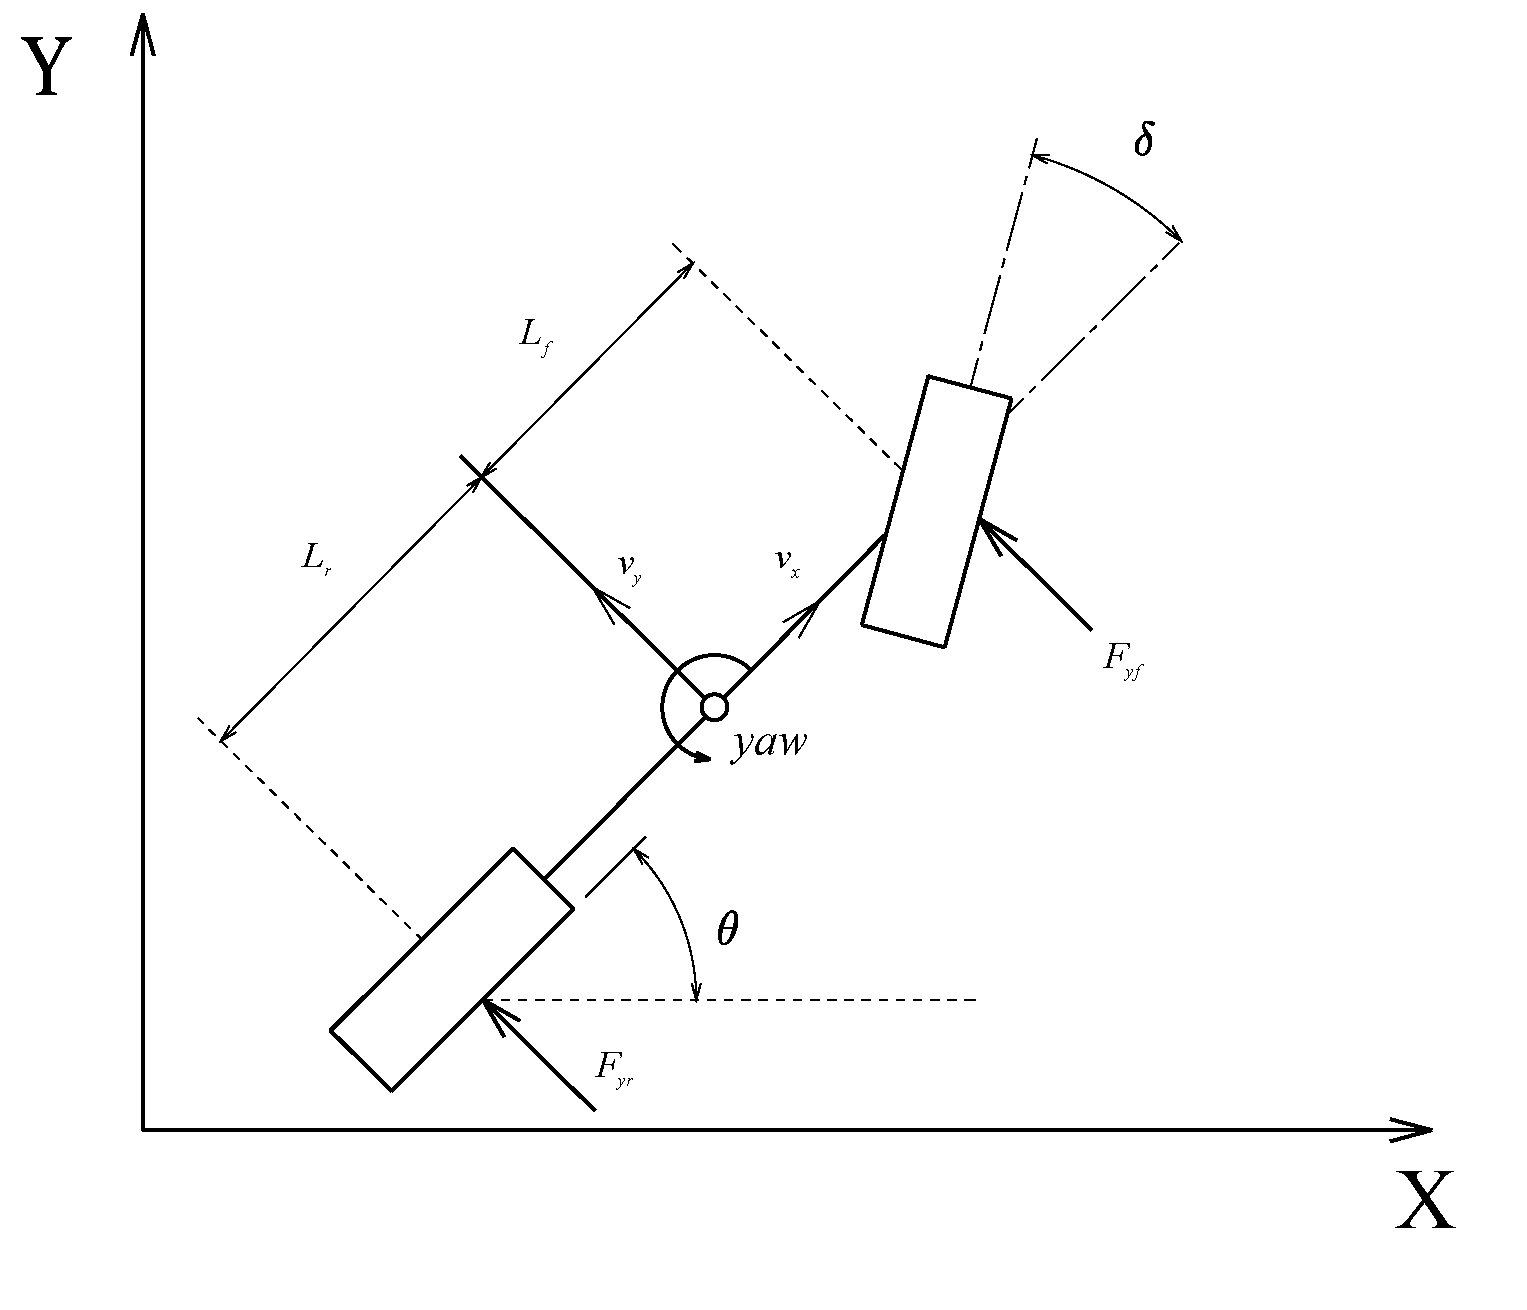
\includegraphics[width=.55\textwidth]{single_track}
\end{center}
}\hfill
\parbox{.4\textwidth}{%
\begin{align*}
  \frac{dx}{ds} &= \cos(\theta) &   \frac{ds_{r}}{ds} &= 1 +
                                                     \frac{W}{2L}\tan(\delta)\\
  \frac{dy}{ds} &= \sin(\theta) & \frac{ds_{l}}{ds} &= 1 -
                                                     \frac{W}{2L}\tan(\delta)\\
  \frac{d\theta}{ds} &= \frac{1}{L}\tan(\delta)\\
  y_{r} &= s_{r} & y_{l} &= s_{l}
\end{align*}}

\noindent For right or left tick
\begin{equation*}
  ds = \frac{2\pi\,r}{10}\frac{1}{1 + \frac{W}{2L}\tan(\delta)}\quad
  \text{or} \quad
  ds = \frac{2\pi\,r}{10}\frac{1}{1 - \frac{W}{2L}\tan(\delta)}
\end{equation*}

If, for any tick, keep track of $d(s_{r}-s_{l})$
\begin{equation*}
  d(s_{r}-s_{l}) = \frac{W\tan(\delta)}{L}ds
\end{equation*}

Euler, 1 wheel encoder (right)
\begin{align*}
  x_{k+1} &= x_{k} + ds_{k}\cos(\theta_{k})\\
  y_{k+1} &= y_{k} + ds_{k}\sin(\theta_{k})\\
  \theta_{k+1} &= \theta_{k} + ds_{k}\frac{1}{L}\tan(\delta_{k})\\
  ds_{k} &= \frac{2\pi\,r}{10}\frac{1}{1 + \frac{W}{2L}\tan(\delta_{k})}  
\end{align*}


\end{document}

%%% Local Variables:
%%% mode: latex
%%% TeX-master: t
%%% End:
